\documentclass[a4paper,11pt,twoside,openright]{scrbook}

\usepackage{swThesis}
\usepackage{amsmath}
\usepackage{standalone}
\usepackage{xcolor}
\standalonetrue

\bibliography{bibliography}

% Figures
\graphicspath{./figs}

\begin{document}

% basically the TCCS book chapter, but with more of an introduction

% compare other methods, PCA, cosine distance etc.

%\printbibliography

\chapter{Measuring distinct phenotypic response} \label{chapter:tccs}

\scriptsize{Note: this chapter is based on previously published work: \textit{"Development of the Theta Comparative Cell Scoring Method to Quantify Diverse Phenotypic Responses Between Distinct Cell Types", S Warchal, J Dawson, N.O Carragher. ASSAY and Drug Development Technologies, pages 395-406, 7:14, 2016.} and \textit{"High-Dimensional Profiling: The Theta Comparative Cell Scoring Method", Phenotypic Screening. Methods in Molecular Biology 1787, 171-181}.} 



\section{Introduction}
\normalsize
\subsection{Comparing response to small molecules across a panel of cell lines}
% First introduce why you would want to compare phenotypic response between cell
% lines
Comparative analysis of cell line panels treated with compounds are routinely used in pharmacogenomic studies and drug sensitivity profiling.
These studies often use large numbers of cell lines and simple measures of compound response such as growth inhibition or cell death, allowing researchers to interrogate sensitivity of various small molecule therapies in a number of genomic backgrounds representing different diseases, disease-subtypes or patient populations.

Using high-content imaging methods with cell line panels enables more complex cellular readouts than cell death resulting in a more detailed characterisation of compound effect.
However, in order to apply multiparametric high-content data to pharmacogenomic studies, there needs to be a robust -- and ideally univariate -- measure of compound response to correlate drug sensitivity with genomic or proteomic datasets.


\subsection{Quantifying compound response in high content screens}
A simple but effective method to quantify the magnitude of compound response from multiparametric data is to calculate the distance from the negative control to the compound induced phenotype in feature space.
This idea was first demonstrated by Tanaka \textit{et al.} using PCA to reduce the dimensionality of a high content screening dataset to 3 principal components, and taking the distance from the centroid of the negative control replicates to the compound co-ordinates. \cite{Tanaka2005}
The distance from the negative control in PCA space is an effective metric for detecting phenotypically active compounds.
In addition, distance measurements can be repeated for multiple concentrations of a compound to produce a concentration -- phenotypic-distance response curve (see figure \ref{figure:pca_dist}) and EC$_{50}$ values.
However, one issue in calculating the distance-from-negative-control metric of compound activity is that it disregards much of the information relating to the position in feature space, as depicted in figure \ref{figure:pca_dist}, two compounds may have similar distances yet those distances may be produced by very different morphological changes.
In order to discern between two such compounds there needs to be a measure of directionality.

\begin{figure}
    \captionsetup{width=0.8\textwidth}
    \caption[Compound distance in principal component space]{
    Diagram illustrating measuring magnitude of compound response by distance from the negative control centroid in principal component space.
    \textbf{(A)} Phenotypic distance to three different compounds.
    Compound A and B show phenotypic activity as they are distanced from the negative control cluster, whereas compound B shows little activity.
    Note that compound A and compound C have similar distances from the negative control centroid, yet have very different values in principal component space.
    \textbf{(B)} A titration series for each of the three compounds, showing how increasing concentrations of compounds A and C show increasing distance from the negative control, whereas weakly active compound C does not increase in distance.
}
    \input{figs/ch3PcaDist.pdf_tex}
    \label{figure:pca_dist}
\end{figure}

% TODO: maybe more info on principal components, eigen vectors?




\section{Results}

\subsection{Compound titrations produce a phenotypic `direction'}
 
Visualising high-content imaging data from compound screens in principal component space reveals a number of patterns and produves a representation of the overall structure of the dataaet.
Performing PCA on morphological feature data from 24 compounds representing 9 mechanistic classes and plotting the first 2 principal components reveals compounds with the same MoA tend to cluster with one another in PCA space (figure \ref{figure:pca_clustering}).

\begin{figure}
    \captionsetup{width=0.8\textwidth}
    \caption[PCA compound clustering based on MoA]{
MoA clustering of compounds based on PCA of their morphological features. 
Principal components calculated from morphological features of 24 compounds grouped into 8 mechanistic classes.
\textbf{(A)} Principal components calculated from an image average of individual cell measurements.
\textbf{(B)} Each point reprensents a well average from individual cell measurements as each well contains 9 image sites.
STS: staurosporine.
}
    \input{figs/ch3pcaClustering.pdf_tex}
    \label{figure:pca_clustering}
\end{figure}

When taking concentrations of compounds into account, is it possible to visualise the effect of increasing concentrations of a compound and how the distance from the negative control and inactive compounds increases.
Figure \ref{figure:pca_direction} shows two highlighted compounds from the same data as in figure \ref{figure:pca_clustering}, we can see as compound concentration increases morphologies become increasingly distant from the untreated negative control cluster positioned centrally, with the two different compounds producing opposite directions.
Mirroring the differences in direction, the morphologies produced by barasertib and cycloheximide are also very different from one another, with barasertib -- an Aurora B kinase -- inhibitor producing large irregular nuclei, and cycloheximide creating small bright nuclei.
This direction in PCA space can be thought of as a phenotypic direction, which can be measured and quantified independent from potency\footnote{as measured by distance from the negative control cluster centroid}.


\begin{figure}
    \captionsetup{width=0.8\textwidth}
    \caption[Two compound titrations highlighted in phenotypic space]{
Principal components of Cellprofiler features calculated from a 24 compound high content screen in MDA-MB-231 cells.
Barasertib (left) and cycloheximide (right) titrations are highlighted to show two active compounds with distinct phenotypes heading in different directions in phenotypic space with increasing concentration.
Images shown next to points are from the Hoechst stain labelling nuclei morphology produced by 1 $\mu$M of each compound.
}
    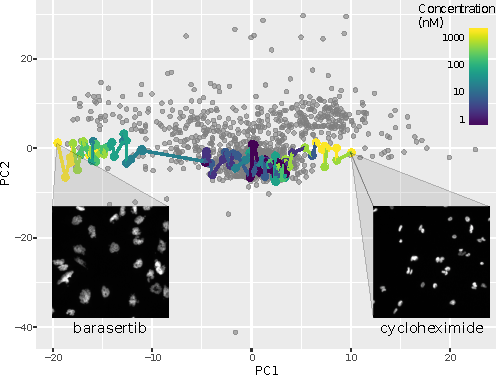
\includegraphics[scale=1.4]{figs/ch3TCCS_direction}
    \label{figure:pca_direction}
\end{figure}


\subsection{Difference in phenotypic direction can be used to quantify distinct phenotypes}

Using direction in addition to distance it is now possible to distinquish between equally phenotypically potent compounds with distinct morphological effects.
By calculating an angle ($\theta$) between phenotypic directions as a function of cosine dissimilarity, a univariate value can be used to quantify phenotypic distance between either different compounds, or cell-lines treated with the same compound to detect distinct phenotypic response.
By calculating $\theta$ against a fixed reference vector, the difference in $\theta$  ($\Delta\theta$) between two treatments can be quantified and visualised in polar co-ordinates as histograms or rose plots (figure \ref{figure:theta_histogram}).
Compounds with the same phenotypic direction will have a small $\Delta\theta$ and compounds with dissimilar phenotypes having a large $\Delta\theta$, when expressed in degrees the values are constrained between 0$^\circ$ and 180$^\circ$.


\begin{figure}
    \captionsetup{width=0.8\textwidth}
    \caption[Visualisation of $\Delta\theta$ to quantify the difference in phenotypic direction between two compounds.]{
Visualisation of $\Delta\theta$ to quantify the difference in phenotypic direction between two compounds.
Histograms in polar co-ordinates show the $\theta$ values of treatments against a fixed reference vector, with $\Delta\theta$ calculated as the difference between the average $\theta$ (black lines) of each compound.
}
    \input{figs/ch3thetaHistogram.pdf_tex}
    \label{figure:theta_histogram}
\end{figure}

Although the data in figures \ref{figure:pca_direction} \& \ref{figure:pca_clustering} show the negative control points clustered near the origin (0, 0) in principal component co-ordinates this is not guaranteed and should not be relied upon, so it is necessary to translate the principal components co-ordinates so that the negative control centroid is position over the median.
In addition, inactive compounds will be positioned in proximity to the negative control points and calculated $\theta$ values will be misleading, therefore removing inactive compounds based on distance from the negative control is an important pre-processing step.


\subsection{SN38 elicits a disinct phenotypic response between cell lines}



\begin{figure}
    \captionsetup{width=0.8\textwidth}
    \caption[Visualisation of $\Delta\theta$ to quantify the difference in phenotypic direction between cell lines]{
Visualisation $\Delta\theta$ to quantify the difference in phenotypic response between cell lines when treated with barasertib.
\textbf{(A)} Ciricular histogram of $\theta$ values of barasertib calculated for eight cell lines.
\textbf{(B)} Phenotypic direction of cell lines treated with barasertib stratified by cell line.
\textbf{(C)} Representation of $\Delta\theta$ for the difference between HCC1569 and MDA-MB-231 cell lines. Note that in this case $\Delta\theta$ is relatively small.
}
    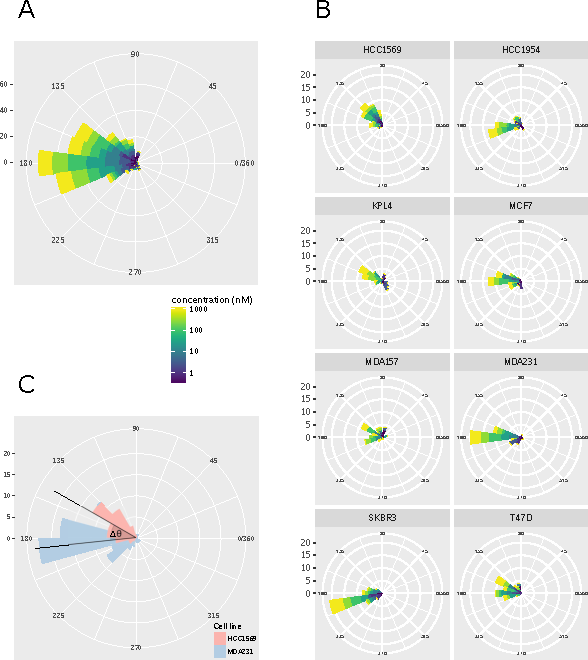
\includegraphics[scale=1.15]{figs/ch3tccsCellLines}
    \label{figure:theta_cell_lines}
\end{figure}

Instead of calculating $\Delta\theta$ between compounds it is also possible to calculate $\Delta\theta$ between cell lines per compound.
To identify and quanitfy differential phenotypic responses, $\Delta\theta$ was calculated between pairs of 8 breast cancer cell lines treated with 24 small molecules at the three highest concentrations (0.1 $\mu$M, 0.3 $\mu$M, 1 $\mu$M).
21 out of the 24 compounds were found to be sufficiently active across the 8 cell lines to proceed, and the difference in phenotypic direction was calculated for all pairs of cell lines for each compound.
Figure \ref{figure:theta_24} shows a heatmap of the calculated $\Delta\theta$ values.
Some compounds such as the Aurora B inhibitors ZM447439 and barasertib showed very little difference in phenotypic response between the breast cancer cell lines, whereas compounds such as the topoisomerase I inhibitor SN38 demonstrated a single cell-line (KPL4) having a distinct response compared to the 7 others.
Particularly striking is the difference between the MCF7 and KPL4 cell lines with a $\Delta\theta$ of 179$^\circ$, indicated near opposite phenotypic responses between the pair of cell lines to the topoisomerase I inhibitor.



\begin{figure}
    \captionsetup{width=0.8\textwidth}
    \caption[Heatmap of $\Delta\theta$ between pairs of cell lines for separate compounds]{
Heatmap of $\Delta\theta$ values between pairs of cell lines for separate compounds.
\textbf{(A)} $\Delta\theta$ calculated between pairs of cell lines treated with 21 compounds as 1 $\mu$M concentration.
Images show differential response between KPL4 and MCF7 cell lines treated with 1 $\mu$M SN38.
    MCF7 cells are observed to decrease in cell area with bright staining for the endoplasmic reticulum, whereas KPL4 cells produce a `fried egg' morphology with large spread cells and weak endoplasmic reticulum staining. Channels used are as follows: \textit{Red} - MitoTracker DeepRed (mitochondria); \textit{Green} - Concanavalin A (endoplasmic reticulum); \textit{Blue} - Hoechst33342 (nuclei). Scale bar: 100 $\mu$m.
\textbf{(B)} Histogram of $\theta$ values calculated for MCF7 and KPL4 cells treated with 1 $\mu$M SN38. $\Delta\theta = 179^\circ$
}
    \includegraphics[scale=1.0]{figs/ch3theta24}
    \label{figure:theta_24}
\end{figure}



\section{Discussion}

% the use of this method, define TCCS
A number of methods exist to classify drug MoA and profile drug response in the context of high-content imaging studies, most of these have only been applied to a single cell type.
The method described in this chapter, named as theta comparative cell scoring (TCCS), was developed to provide a pragmatic way to perform comparative high-content imaging studies across genetically and morphologically distinct cell lines.
TCCS should be viewed as an extension to the common distance-in-PCA approach taking directionality into consideration in addition to distance from controls.
The benefits of TCCS over previous methods are as follows: (1) the use of distance from the negative control to remove inactive compounds as one of the first steps prevents spurious differences that would be present in measures such as correlation or simple cosine similarity; (2) The comparison of each data point to a common reference vector enables visulisation of a phenotypic direction.


\begin{figure}
    \captionsetup{width=0.8\textwidth}
    \caption[TCCS workflow]{
Theta comparative cell scoring (TCCS) workflow.
\textbf{(A)} Normalised and standardised numerical data.
    \textbf{(B)} Principal component analysis, negative control values coloured in blue.
    \textbf{(C)} Centering of principal component values to the negative control centroid.
    \textbf{(D)} Calculation of distance from the origin to each data point, an activity cutoff is derived fro the standard deviation of the distance to the negative control values.
    \textbf{(D.2)} In two-dimensional space, a directional histogram can be created by the angle of each vector against a reference vector.
    \textbf{(E)} Inactive compounds excluded based on distance from the origin.
    \textbf{(F)} Determining the angle between compounds/cell-lines.
    \textbf{(F.2)} Visualisation or clustering of compounds based on $\theta$ values.
}
    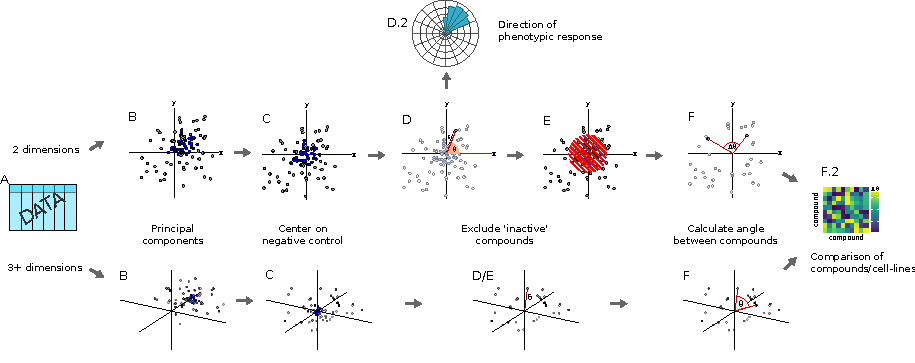
\includegraphics[scale=1.0]{figs/ch3thetaWorkflow}
    \label{figure:theta_workflow}
\end{figure}

% importance of normalisation to remove cell-line specific morphologies before
% PCA
When comparing compound response between cell lines the most critical step, regardless of subsequent methods, is to account for the inherent morphological differences between untreated cell lines.
Without this normalisation step morphologically distinct cell lines are not directly comparable as their large scale morphological differences will mask any difference in morphological response to a compound.

% issue of potency, inactive compound in one cell-line might mean the compound
% is removed from the analysis when this is an interesting results -- need to
% pre-analyse with phenotypic distance to find these hits.
The TCCS method removes compounds which are deemed to be inactive if they are not sufficiently distant from the negative control (see figure \ref{figure:theta_workflow}).
While this increases the robustness of the calculation by removing spurious differences in direction, it also introduces a new problem when compounds elicit large differences in potency between cell lines.
This would result in the removal of such compounds from the analysis despite producing a genuine, and potentially biologically interesting, differential response between cell lines.
This can be rectified by identifying these compounds when computing compound distances from the negative control in principal component space -- any compounds that show large differences in this distance between cell lines can be flagged for further analysis before removal.


% 2 principal components might not capture all the variation in the data, method
% works in higher dimensions
When using high-content imaging data with a lot of morphological feature measurements, using the first two principal components as depicted in this chapter may only account for a small proportion of variation in the data.
This may lead to potentially missing interesting differences which are only evident in later principal components.

Fortunately, as part of the TCCS algorith the cosine similarity equation uses the dot product of the two vectors reducing any two equal length vectors to a single number, enabling the use of 3 or more principal components.
Therefore the proportion of variance to keep in the data can be specified beforehand, and the dimensionality of the data reduced in a way to suit the statistical properties of different datasets.

% relating phenotypic direction back to principal component feature weightings
% to make result more interpretable -- using other dimensional reduction
% techniques might make this easier
An interesting prospect of `phenotypic direction' is relating directions back to combinations of morphological features to provide more interpretability to the results.
This is possible with PCA by using the feature loadings describe the contributions of original features used to construct each principal component.
However, as PCA uses arbitrary positive and negative weights for these feature loadings, other dimensional reductions techniques might be better suited for generating more interpretable results.
One example is non-negative matrix factorisation which would return only positive weights for the morphological features, making the contribution of morphological features to the phenotypic direction more interpretable.


% using multiple concentrations
Multiple concentrations are not often used in high throughput cell based screening assays despite providing useful information to detect off-target effects as well as reducing false negatives by screening at incorrect concentrations.
A potential improvement of the TCCS method is to incoporate data from compound titrations as in figure \ref{figure:pca_direction} and fitting a linear model to the data points providing information relating to goodness of fit.
This could potentially be used to identify compounds with off-target effects at higher concentrations if they do not fit a linear model well which indicates the data points going off at a tangent at higher concentrations towards phenotypic space indicative of cell death (e.g figure \ref{figure:pca_dist} B compound A).

% summary of summary
In conclusion, the TCCS method presents an alternative to (dis)similarity measures such as correlation and cosine distance with important prior steps to account for perculiarities in high-content screening data, enabling high-content screening studies for quantifying distinct phenotypic response between morphologically diverse cell types.
% TODO: expand this


\section{Methods}

\subsection{Data pre-processing}
Tabular data from Cellprofiler measuring 309 morphological features for each cell was aggregated to an image median.
To remove batch effects and to remove inherent cell-line specific morphologies data was normalised by dividing each morphological feature by the median negative control value for that feature per plate.
Each feature was then standardised to a mean of zero and unit variance on the pooled data.

\subsection{Principal component analysis}

Principal components were calculated using the \texttt{prcomp} function in R v3.2, with no centering or scaling as this was performed manually beforehand.

\subsection{Selecting the number of principal components}
The number of principal components to used in the analysis can be determined by specifying beforehand the proportion of variance in the data that should be kept, and then finding the minimum number of principal components that account for that proportion of variance in the dataset.

E.g in R:

\begin{minted}[mathescape,
linenos,
numbersep=5pt,
fontseries=Roboto Mono Medium,
fontsize=\footnotesize,
gobble=4,
frame=leftline,
framesep=2mm]{r}
    threshold = 0.8
    pca_output = prcomp(data)
    pc_variance = pca_output$stdev^2 
    cumulative_prop_variance = cumsum(pc_variance) / sum(pc_variance)
    n_components = min(which(cumulative_prop_variance >= threshold)) 
\end{minted}
where \texttt{data} is numeric dataframe of morphological features.


\subsection{Centering the data on the negative control}

In order to centre the principal component data so that the mediod of the negative control was positioned on the origin, the median value for each feature columns for the negative control data was calculated.
Then finding how much this differs from the origin for each feature, all principal component values were adjusted by this difference.

\begin{enumerate}
    \item Calculate the median value $m$ for each principal component for the negative control data (medioids).
    \item Subtract each medioid from 0 in order to find the difference from the origin to $\delta m_i$, where $i$ is the $i^{th}$ principal component.
    \item Add $\delta m_i$ to each value in the $i^{th}$ principal component.
\end{enumerate}

For example in R, given a dataframe \texttt{data} containing a metadata column \texttt{"compound\_name"} of compound names, with \texttt{"DMSO"} as a negative control, and \texttt{feature\_cols} as a list of non-metadata column names:


\begin{minted}[mathescape,
linenos,
numbersep=5pt,
fontseries=Roboto Mono Medium,
fontsize=\footnotesize,
gobble=4,
frame=leftline,
framesep=2mm]{r}
    mediods = apply(data[data[, "compound_name"] == "DMSO"], 2, median)
    delta_m = 0 - mediods # $\delta m$
    for (i in seq_along(feature_cols)) {
        feature = feature_cols[i]
        # feature_column$_i$ $:=$ feature_column$_i$ + $\delta m_i$
        data[, feature] = data[, feature] + delta_m[i]
    }
\end{minted}


\subsection{Identifying inactive compounds}

Inactive compounds were identified by determining a minimum cut-off distance to the negative control centroid in principal component space.
This was calculated by first finding the $l_1$ norm\footnote{A.K.A Manhattan or city-block distance} from each compound at all concentrations to the negative control centroid.
The standard deviation of all these distances was calculated and any compound which was within 2 standard deviations of the negative control centroid at 1 $\mu$M was deemed inactive, if a compound was found to be inactive in any one of the eight cell lines it was removed from the analysis.


\subsection{Calculating $\theta$ and $\Delta\theta$}

$\theta$ was calculated by taking cosine dissimilarity between two vectors ($u$ and $v$) in principal component space and coverting into degrees.

\begin{equation} \label{equation:theta}
        \theta = \cos^{-1} \left( \frac{u \cdot v}{||u||v||} \right) \cdot \frac{180}{\pi}
\end{equation}

When $v$ is a common fixed reference vector, $\Delta\theta = |\theta_i - \theta_j|$ where $\theta_i$ and $\theta_j$ are theta values for 2 vectors.
As opposite phenotypic directions are at 180$^\circ$, $\Delta\theta$ values greater than 180$^\circ$ should be thought as converging towards similar phenotypes.
Therefore $\Delta\theta$ values were constrained to a maximum value of 180$^\circ$ by substracting any value greater than 180$^\circ$ from 360.

\begin{equation}
\theta = 
    \begin{cases}
        360 - \theta & \text{if } \theta > 180\\
        \theta       & \text{otherwise}
    \end{cases}
\end{equation}

\end{document}



